\documentclass[11pt]{scrartcl}

\usepackage{natbib}
\usepackage{amsmath}

\usepackage{amsthm}
\newtheorem{remark}{Remark}

\usepackage{hyperref}

\usepackage{booktabs}
\usepackage{multirow}
\usepackage{graphicx}

\usepackage[ruled,linesnumbered,boxed]{algorithm2e}

\title{DKAN: Kolmogorov-Arnold Networks with Dynamic Grids}
\author{
	Ziyang Gong\thanks{Email: gongziyang@smail.swufe.edu.cn} \\
Center of Statistical Research and School of Statistics\\
 Southwestern University of Finance and Economics, Chengdu, China
}
\date{}

\begin{document}
\maketitle

\begin{abstract}
	The recently proposed Kolmogorov-Arnold Networks (KANs) have shown promising results in approximating continuous functions using B-splines. However, the predefined grids in KANs may not align well with the input activations, leading to suboptimal performance. In this paper, we proposed Kolmogorov-Arnold Networks with Dynamic Grids (DKANs), a novel neural network architecture that leverages dynamic grid selection to improve the performance of KANs. By dynamically adjusting the grid points based on the distribution of input activations, DKANs can better align with the data, leading to more accurate modeling and analysis. We demonstrated the effectiveness of DKANs through experiments on synthetic and real-world datasets, showcasing superior performance compared to KANs.\\
	\textbf{Keywords:} Kolmogorov-Arnold Networks, B-splines, Grids Selection.
\end{abstract}

\section{Introduction}

Recently, \citet{liu2024kan} proposed Kolmogorov-Arnold Networks (KANs), a novel class of neural network architectures inspired by the work of Andrey Kolmogorov and Vladimir Arnold on representing continuous functions using a sum of simple functions. The core idea behind KANs is to represent a multivariate function $f(\mathbf{x})$ as a superposition of simpler functions, which can be more easily learned by a neural network. Specifically, a KAN represents a function $f(\mathbf{x})$ as
\begin{equation}
	f(\mathbf{x}) = \sum_{q} \Phi^{q}\left(\sum_{p} \phi_{q,p}\left(x_{p}\right)\right),
\end{equation}
where $\Phi$ and $\phi$ are univariate functions. This hierarchical structure allows KANs to model complex functions by decomposing them into simpler components, which can be learned more efficiently by the network.
To define the family of functions for $\Phi$ and $\phi$, \citet{liu2024kan} utilized B-splines, which are theoretically capable of approximating any smooth univariate function within a given interval.

In non-parametric estimation, splines are commonly employed tools, and the grids are typically selected based on the quantiles of the input data or by equally spacing the interval of the input data.
However, in the context of KANs, the input activations are not directly observable, during the training stage the input activations can shift out of the predefined grids, potentially leading to suboptimal performance.
\citet{liu2024kan} acknowledged this issue and proposed a solution that rescales the grids when the input activations shift out of the predefined grids; however, this rescaling can lead to severe efficiency bottlenecks in KANs.
To address this, \citet{li2024kolmogorov} used Gaussian radial basis functions (RBFs) to approximate the activation functions in KANs, which can be considered an approximation of the B-spline basis functions and showed that the calculation efficiency of KANs can be significantly improved by using RBFs.

In this paper, we propose Dynamic KANs (DKANs), where the grid points are dynamically selected based on the distribution of the input activations. By analyzing the distribution of these activations, our method adjusts the grid points in real-time, ensuring better alignment and improving the performance of the network. This approach addresses the challenge identified by \citet{liu2024kan} and provides a theoretically grounded framework for optimal grid updates.

\section{Preliminaries}

\paragraph*{Construction of B-spline basis functions}

Suppose we have $m$ $(m\geq 0)$ distinct internal knots, $\xi_1, \ldots, \xi_m$, placed within the boundary knots $a$ and $b$, satisfying $a<\xi_1<\cdots<\xi_m<b$. We can define $t_1=\cdots=t_d=a$, $t_{d+j}=\xi_j$ for $j \in\{1, \ldots, m\}$, and $b=t_{d+m+1}=\cdots=t_{d+p}$, where $k$ and $d=k+1$ represent the polynomial degree and the order of a basis function, respectively, and $p=d+m$ represents the degrees of freedom of a basis function. Given internal knots, $\xi_1, \ldots, \xi_m$, and boundary knots, $L$ and $U$, the simple knot sequence intended for splines of degree $k$ is denoted by $\mathbf{T}_k$.
For a given degree of splines $k \in$ $\{1,2, \ldots\}$, the $i$ th B-spline basis of degree $k$ (or order $d=k+1$ ) denoted by $B_{i,k}(x)$ based on the simple knot sequence $\mathbf{T}_k$ can be defined by the following Cox-de Boor recursive formula:
\begin{equation*}
	B_{i,k}\left(x \mid \mathbf{T}_k\right)=\left(\frac{x-t_i}{t_{i+k}-t_i}\right) B_{i, k-1}\left(x \mid \mathbf{T}_k\right)+\left(\frac{t_{i+k+1}-x}{t_{i+k+1}-t_{i+1}}\right) B_{i+1, k-1}\left(x \mid \mathbf{T}_k\right),
\end{equation*}
with
\begin{equation*}
	B_{l,0}\left(x \mid \mathbf{T}_k\right)=\left\{\begin{array}{ll}
		1, & t_l \leq x<t_{l+1}  \\
		0, & \text { otherwise }
	\end{array}, l \in\{1, \ldots, d+p-1\}\right.,
\end{equation*}
where $L \leq x<U, p=m+d$ represents the degrees of freedom, and $i \in\{1, \ldots, p\}$.
For simplicity, we will abbreviate $B_{i,k}(x \mid \mathbf{T}_k)$ as $B_{i}(x)$ in the following text.

\paragraph*{Kolmogorov-Arnold Networks}

A general KAN network consisting of $L$ layers takes $\mathbf{x}$ to generate the output as:
\begin{equation}
	\label{eq:general-KAN}
	\operatorname{KAN}(\mathbf{x})=\left(\Phi^{(L-1)}\circ\Phi^{(L-2)}\circ\cdots\circ\Phi^{(1)}\circ\Phi^{(0)}\right)\mathbf{x}
\end{equation}
which $\Phi^{(l)}$ is the function matrix of the $l^{\text{th}}$ KAN layer or a set of pre-activations. Let denote the neuron $i^{\text{th}}$ of the layer $l^{\text{th}}$ and the neuron $j^{\text{th}}$ of the layer $l+1^{\text{th}}$. The activation function $\phi_{ij}^{(l)}$ connects $(l,i)$ to $(l+1, j)$:
\begin{equation*}
	\phi_{ij}^{(l)},\quad l=0, \cdots, L-1, \quad i=1, \cdots, n_l,\quad j=1, \cdots, n_{l+1}
\end{equation*}
with $n_l$ is the number of nodes of the layer $l^{t h}$. So now, the function matrix $\Phi^{(l)}$ can be represented as a matrix $n_{l+1}\times n_l$ of activations:
\begin{equation*}
	\Phi^{(l)}=\left(\begin{array}{cccc}
			\phi_{11}^{(l)}(\cdot)       & \phi_{12}^{(l)}(\cdot)       & \cdots & \phi_{1n_l}^{(l)}(\cdot)       \\
			\phi_{21}^{(l)}(\cdot)       & \phi_{22}^{(l)}(\cdot)       & \cdots & \phi_{2n_l}^{(l)}(\cdot)       \\
			\vdots                       & \vdots                       & \vdots & \vdots                         \\
			\phi_{n_{l+1}1}^{(l)}(\cdot) & \phi_{n_{l+1}2}^{(l)}(\cdot) & \cdots & \phi_{n_{l+1}n_l}^{(l)}(\cdot)
		\end{array}\right).
\end{equation*}
The activation function $\phi$ is the sum of basis function $b(x)$ and the spline function $\text{spline}(x)$:
\begin{equation}
	\phi(x)=w(b(x)+\text{spline}(x)),
\end{equation}
where $w$ is the scaling factor, $b(x)$ is set as $b(x)=\text{silu}(x)=x/(1+\exp(-x))$, and in most cases, the spline function $\text{spline}(x)$ is parameterized as a linear combination of B-spline basis functions:
\begin{equation*}
	\text{spline}(x)=\sum_{k}c_kB_k(x).
\end{equation*}
In the above equation, both $w$ and $c_k$ are learnable parameters.

\section{Method}

\paragraph*{Selection of grid points}

The intuitive approach assumes that the input activations follow a normal distribution, which can be represented as:
\begin{equation}
	z_{ij}^{(l)} \sim \mathcal{N}\left(\mu_{ij}^{(l)}, \sigma_{ij}^{(l)2}\right),
\end{equation}
where $z_{ij}^{(l)}$ is the output activation from $i^{\text{th}}$ neuron in the $l-1^{\text{th}}$ layer to the $j^{\text{th}}$ neuron in the $l^{\text{th}}$ layer, and $\mu_{ij}^{(l)}$ is the mean, and $\sigma_{ij}^{(l)2}$ is the variance of the normal distribution for the $i$-th activation of the $j$-th neuron.

To accurately capture the behavior of these activations, we determine the grid points based on the quantiles of the normal distribution. Specifically, the grid points $\zeta_{ij,k}^{(l)}$ are computed as:
\begin{equation}
	\zeta_{ij,k}^{(l)}=\mu_{ij}^{(l)}+\sigma_{ij}^{(l)}\Phi^{-1}\left(\alpha+\frac{k}{K}(1-2\alpha)\right),\quad k=1,\ldots,K,
\end{equation}
where $\Phi^{-1}(\cdot)$ represents the inverse of the standard normal cumulative distribution function, $\alpha$ is a small constant introduced to prevent the quantiles from reaching infinite values, and $K$ is the total number of grid points. The boundaries of these grid points are defined as follows:
\begin{equation}
	a=\mu_{ij}^{(l)}+\sigma_{ij}^{(l)}\Phi^{-1}(\alpha),\quad b=\mu_{ij}^{(l)}+\sigma_{ij}^{(l)}\Phi^{-1}(1-\alpha),
\end{equation}
where $a$ and $b$ denote the lower and upper boundaries of the grid points, respectively. This ensures that the grid covers the central region of the distribution, avoiding extremes that could lead to numerical instability.

By utilizing this approach, we can systematically and effectively discretize the input activations into grid points that reflect the underlying normal distribution. This method not only simplifies the computational complexity but also preserves the statistical properties of the activations, enabling more accurate modeling and analysis.

\begin{remark}
	However, there remains the issue that the input activations may fall outside the boundaries of the grid points, resulting in the loss of information from these activations. To address this problem, we introduce two additional basis functions, $B_{0}(x) = \max(0, -x + a)$ and $B_{K+1}(x) = \max(0, x - b)$, to capture the information of the input activations that lie outside the boundaries of the grid points.
\end{remark}

With the pre-defined grid points $\zeta_{ij,k}^{(l)}$ and the additional basis functions, the B-spline function's basis functions are shown in Figure~\ref{fig:activation-function}.

\begin{figure}[htbp]
	\centering
	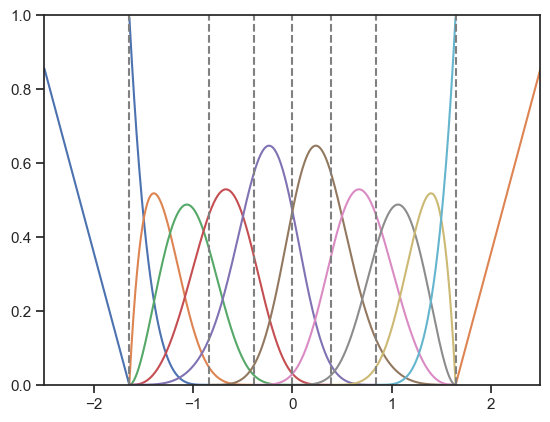
\includegraphics[width=0.5\textwidth]{figures/dkan-splines.png}
	\caption{The basis functions of the DKAN's spline function with $K=5$ grid points, and $\alpha=0.05$, given that the input activations follow a standard normal distribution.}
	\label{fig:activation-function}
\end{figure}

Thus, the activation function $\phi$ can be represented as:
\begin{equation}
	\phi(x)=wb(x)+\sum_{k=0}^{K+1}c_{k}B_{k}(x),
\end{equation}
where $b(x)$ is the silu function, both $w$ and $c_{k}$ are the learnable parameters, and $B_{k}(x)$ are the basis functions of the B-spline function defined by the grid points $\zeta_{ij,k}^{(l)}$. Here, we absorb the scaling factor $w$ into the basis functions to simplify the notation.

Compared to the B-spline basis functions in \citet{liu2024kan}, the key differences can be summarized as follows:
\begin{enumerate}
	\item The grid points are dynamically selected based on the distribution of the input activations, rather than being predefined, ensuring better alignment with the data.
	\item Additional basis functions, $B_{0}(x)$ and $B_{K+1}(x)$, are introduced to capture information from input activations that fall outside the boundaries of the grid points.
\end{enumerate}

\paragraph*{Estimation of the mean and variance}

The remaining question is how to estimate the parameters $\mu_{ij}^{(l)}$ and $\sigma_{ij}^{(l)2}$ during the training process. For ease of presentation, we simplify $\mu_{ij}^{(l)}$ and $\sigma_{ij}^{(l)2}$ as $\mu$ and $\sigma^{2}$, respectively.
Inspired by the batch normalization method proposed by \citet{ioffe2015batch}, we introduce a straightforward approach that utilizes the moving average of the input activations. Specifically, we maintain a moving average for both the mean and variance of the input activations, denoted as $\widehat{\mu}$ and $\widehat{\sigma}^{2}$, respectively. These moving averages are updated iteratively during training using the following equations:
\begin{equation}
	\widehat{\mu} \leftarrow (1 - \gamma)\widehat{\mu} + \gamma\widehat{\mu}_{\mathcal{B}}, \quad \widehat{\sigma}^{2} \leftarrow (1 - \gamma)\widehat{\sigma}^{2} + \gamma\widehat{\sigma}_{\mathcal{B}}^{2},
\end{equation}
where $\widehat{\mu}_{\mathcal{B}} = \frac{1}{m}\sum_{k=1}^{m}z_{ij,m}^{(l)}$ and $\widehat{\sigma}_{\mathcal{B}}^{2} = \frac{1}{m}\sum_{k=1}^{m}\left(z_{ij,m}^{(l)} - \widehat{\mu}_{\mathcal{B}}\right)^{2}$ represent the batch-wise estimates of the mean and variance, respectively. Here, $m$ is the batch size, and $z_{ij,m}^{(l)}$ denotes the $m$-th input activation in the batch.
The parameter $\gamma$ is known as the momentum term. It plays a crucial role in stabilizing the estimation of $\mu$ and $\sigma^{2}$, preventing rapid fluctuations that could lead to instability in the grid points. By appropriately tuning $\gamma$, we ensure that the moving averages $\widehat{\mu}$ and $\widehat{\sigma}^{2}$ evolve smoothly over time, providing robust estimates that are less susceptible to noise from individual batches.

\paragraph*{DKAN operator}

Within the above framework, we can define the DKAN operator for the $j$-th neuron in the $l$-th layer to the $k$-th neuron in the $l+1$-th layer, as shown in Algorithm~\ref{alg:dkan-operator}.
The DKAN operator in Algorithm~\ref{alg:dkan-operator} is easy to implement and can be integrated into existing neural network architectures. A PyTorch implementation of the DKAN operator is provided in \href{https://github.com/SignorinoY/DKAN}{https://github.com/SignorinoY/DKAN}.

\begin{algorithm}[htbp]
	\caption{DKANs operator for $j$-th neuron in layer $l$ to $k$-th neuron in layer $l+1$.}
	\label{alg:dkan-operator}
	\KwData{Bathched input activations $\left\{\mathbf{z}_{ij}^{(l)}\right\}$, spline degree $p$, number of grid points $K$, quantile $\alpha$, momentum term $\gamma$.}
	Initialize $\widehat{\mu}_{ij}^{(l)} \leftarrow 0$, $\widehat{\sigma}_{ij}^{(l)2} \leftarrow 1$\;
	Initialize the grid points $\{\zeta_{ij,k}^{(l)}\}$, $a$ and $b$ based on the standard normal distribution according to Equations (5) and (6)\;
	\For{each batch $\mathcal{B}$} {
	Update by moving average estimates:
	\begin{equation*}
		\widehat{\mu}_{ij}^{(l)} \leftarrow (1 - \gamma)\widehat{\mu}_{ij}^{(l)} + \gamma\widehat{\mu}_{\mathcal{B}}, \quad \widehat{\sigma}_{ij}^{(l)2} \leftarrow (1 - \gamma)\widehat{\sigma}_{ij}^{(l)2} + \gamma\widehat{\sigma}_{\mathcal{B}}^{2},
	\end{equation*}
	where $\mu_{ij}^{(l)} \leftarrow \frac{1}{m}\sum_{k=1}^{m}z_{ij,m}^{(l)}$, and $\sigma_{ij}^{(l)2} \leftarrow \frac{1}{m}\sum_{k=1}^{m}\left(z_{ij,m}^{(l)} - \mu_{ij}^{(l)}\right)^{2}$\;
	Normalize the input activations $z_{ij}^{(l)}$ based on the $\widehat{\mu}_{ij}^{(l)}$ and $\widehat{\sigma}_{ij}^{(l)2}$
	\begin{equation*}
		z_{ij}^{(l)} \leftarrow \frac{z_{ij}^{(l)} - \widehat{\mu}_{ij}^{(l)}}{\sqrt{\widehat{\sigma}_{ij}^{(l)2}}};
	\end{equation*}
	Compute the output of the DKAN network
	\begin{equation*}
		z_{jk}^{(l+1)}:=\phi_{jk}^{(l+1)}(z_{ij}^{(l)})=w\operatorname{silu}(z_{ij}^{(l)})+\sum_{k=0}^{K+1}c_{k}B_{k}(z_{ij}^{(l)}),
	\end{equation*}
	where $B_{k}(\cdot)$ is the B-spline basis function defined by the grid points $\{\zeta_{ij,k}^{(l)}\}$ and the boundaries $a$ and $b$\;
	}
	\KwResult{Output activations $\left\{\mathbf{z}_{jk}^{(l+1)}\right\}$}
\end{algorithm}

\section{Experiments}

To evaluate the performance of DKANs, we conducted experiments on synthetic and real datasets, comparing the results with those obtained using KANs.
The KAN model was implemented based on the efficient-kan package \cite{blealtan2024blealtan}, and the experiments were conducted using the PyTorch framework \footnote{The code is available at \href{https://github.com/SignorinoY/DKAN}{https://github.com/SignorinoY/DKAN}.}.

\subsection{Synthetic data}

In this study, we consider a simple synthetic dataset to evaluate the performance of DKANs and compare them with KANs, particularly focusing on scenarios where the input activations fall within or outside the predefined grid points used in KANs.

The synthetic dataset consists of 10,000 samples. The covariates were generated under two distinct conditions:
\begin{enumerate}
	\item Inside the predefined interval: The covariates $\mathbf{x}_{i}$ were drawn from a uniform distribution, specifically $x_{i} \sim U(-3, 3)$ for $i=1,2$.
	\item Outside the predefined interval: The covariates $\mathbf{x}$ were sampled from a multivariate normal distribution, $\mathbf{x} \sim \mathcal{N}(\mathbf{0}, \Sigma)$, where the covariance matrix $\Sigma$ is given by:
	      \begin{equation*}
		      \Sigma=\begin{bmatrix}
			      1 & 0 \\
			      0 & 1
		      \end{bmatrix}.
	      \end{equation*}
\end{enumerate}
The response variable $y_i$ was generated using the following non-linear function:
\begin{equation*}
	y_{i} = \log\left(|x_{1}| + (x_{2}/2)^{2} + 1\right) + \varepsilon_{i},\quad \varepsilon_{i} \sim \mathcal{N}(0, 0.1^{2}).
\end{equation*}

Both the KANs and DKANs model architectures were kept consistent across all simulations, i.e., [2, 1, 1]. To ensure a comparable number of parameters, we set the B-spline basis functions to order 3 for both models. The KANs model had 8 grid points, while the DKANs model had 5 grid points. This adjustment accounted for the additional scaling factor $w$ in the KAN model.
The total number of parameters in the KANs and DKANs models was 39 and 40, respectively.
Specifically, the grid boundaries for the KANs model were set to $[-1,1]$, while the grid boundaries for the DKANs model were dynamically selected based on the distribution of the input activations.

During training, we utilized the Adam optimizer with a learning rate of 0.05 and a batch size of 256. Additionally, the training dataset was randomly split into training and validation sets, with 90\% of the data used for training and the remaining 10\% reserved for validation.
The models were trained until the validation loss converged, with early stopping applied to prevent overfitting. This approach ensured that the models did not continue to train once performance on the validation set ceased to improve, thereby enhancing the generalizability of the models.

The experiments were repeated ten times to account for variability in the results. The minimum validation MSE loss and test MSE loss, along with the mean validation MSE loss and test MSE loss (in parentheses), are presented in Table \ref{tab:synthetic-dataset}.

\begin{table}[htbp]
	\centering
	\caption{Comparison of DKANs and KANs on synthetic datasets. The results are presented as the minimum validation and test loss, with the mean validation and test loss provided in parentheses.}
	\label{tab:synthetic-dataset}.
	\begin{tabular}{cccccc}
		\toprule
		Type                     & Method & Validation      & Test            \\
		\midrule
		\multirow{2}{*}{Inside}  & DKAN   & 0.0103 (0.0129) & 0.0103 (0.0133) \\
		                         & KAN    & 0.0101 (0.0106) & 0.0101 (0.0108) \\
		\midrule
		\multirow{2}{*}{Outside} & DKAN   & 0.0112 (0.0180) & 0.0108 (0.0176) \\
		                         & KAN    & 0.0143 (0.0223) & 0.0144 (0.0226) \\
		\bottomrule
	\end{tabular}
\end{table}

Based on the results, we observe that while DKANs can perform comparably to KANs when input activations fall within predefined grid points, however, they exhibit superior performance when input activations fall outside these points. Specifically, DKANs achieve lower validation and test losses in such scenarios. This highlights the effectiveness of the dynamic grid selection approach in DKANs, which allows the model to adapt to the distribution of input activations, leading to more accurate and robust predictions.

\subsection{Real data}

To better understand the performance of DKANs, we conducted a series of experiments using three well-known real-world datasets: MNIST \citep{lecun2010mnist}, FMNIST \citep{xiao2017fashion}, and KMNIST \citep{clanuwat2018deep}. Each dataset consists of 28x28 pixel grayscale images, with each image corresponding to one of 10 distinct classes, and each dataset contains 60,000 images for training and 10,000 images for testing.
% The MNIST dataset contains handwritten digits, providing a classic benchmark for image classification tasks. The FMNIST dataset, or Fashion-MNIST, offers a more challenging alternative with images of various clothing items, pushing the model to distinguish between similar fashion articles. Lastly, the KMNIST dataset includes images of Japanese characters (Kanji), introducing another layer of complexity and diversity to our evaluation.

Both the KANs and DKANs model architectures were kept consistent across all datasets, i.e., [28*28, 64, 10]. The total number of parameters in the KANs and DKANs models was approximately 609,000, respectively. Other settings, such as the optimizer, learning rate, batch size, and training duration, were consistent with the synthetic data experiments.
The experiments for each dataset were repeated ten times to account for variability in the results. The max validation and test accuracies, along with the mean validation and test accuracies in parentheses, are presented in Table \ref{tab:real-datasets}.

\begin{table}[htbp]
	\centering
	\caption{Comparison of DKANs and KANs on real-world datasets. The results are presented as the maximum validation and test accuracies, with the mean validation and test accuracies provided in parentheses.}
	\label{tab:real-datasets}
	\begin{tabular}{cccccc}
		\toprule
		Dataset                 & Method & Validation      & Test            \\
		\midrule
		\multirow{2}{*}{MNIST}  & DKAN   & 0.9678 (0.9641) & 0.9675 (0.9655) \\
		                        & KAN    & 0.9672 (0.9637) & 0.9678 (0.9654) \\
		\midrule
		\multirow{2}{*}{FMNIST} & DKAN   & 0.8930 (0.8890) & 0.8846 (0.8803) \\
		                        & KAN    & 0.8917 (0.8873) & 0.8815 (0.8768) \\
		\midrule
		\multirow{2}{*}{KMNIST} & DKAN   & 0.9428 (0.9383) & 0.8616 (0.8553) \\
		                        & KAN    & 0.9348 (0.9310) & 0.8553 (0.8506) \\
		\bottomrule
	\end{tabular}
\end{table}

The results demonstrate that DKANs consistently outperformed KANs across all datasets, achieving higher validation and test accuracies. However, an exception was observed in the mean validation accuracy for the KMNIST dataset, where the KANs model outperformed the DKANs model. This discrepancy may be attributed to the complexity of the KMNIST dataset, which contains a diverse range of Japanese characters that are more challenging to classify accurately. Nevertheless, the overall trend indicates that DKANs offer improved performance compared to KANs, highlighting the effectiveness of the dynamic grid selection approach.

\section{Conclusion}

The recently proposed KANs have brought renewed attention to the classical non-parametric estimation tools, B-splines, within the context of deep learning. Despite their potential, the use of B-splines in KANs also introduces challenges such as increased computational complexity and reduced efficiency compared to multi-layer perceptrons.
In this paper, we address the issue of predefined grids in KANs, which may not align well with the distribution of input activations, potentially leading to suboptimal performance. To overcome this limitation, we propose Kolmogorov-Arnold Networks with Dynamic Grids, which are designed to enhance the performance of KANs through dynamic grid selection.
Our proposed DKANs architecture not only addresses the inherent limitations of predefined grids but also demonstrates the potential for broader applications where dynamic adjustment can lead to significant improvements in deep learning models. Through a series of experiments on real-world datasets, we show that DKANs consistently outperform KANs, validating the effectiveness of our approach in achieving more accurate and robust neural network models

\bibliography{references}
\bibliographystyle{apalike}

\end{document}
